\documentclass[english]{article}
\usepackage[letterpaper]{geometry}
\usepackage{hyperref}
\usepackage{graphicx}
\usepackage{caption}
\usepackage{subcaption}
\usepackage{epstopdf}
\usepackage{float}
\geometry{verbose,tmargin=1in,bmargin=1in,lmargin=1in,rmargin=1in}

\newcommand{\nb}{Na\"ive Bayes}
\newcommand{\matlab}{\textsf{MATLAB}}
\newcommand{\liblinear}{\textsf{LIBLINEAR}}

\begin{document}

\title{CIS 520 Final Project Report: Team Kernel Sanders}
\author{
  Brendan Callahan\\
  \texttt{bcal@seas.upenn.edu}
  \and
  Patrick Crutchley\\
  \texttt{pcrutchl@psych.upenn.edu}
  \and
  Michael Woods\\
  \texttt{micwoods@mail.med.upenn.edu}
}
\date{December 10, 2013}

\maketitle

\section{Background}
The competition this year focused on developing a method of sentiment analysis for user reviews of restaurants and other businesses from a supplied Yelp dataset. As participants, the task laid before us was conceptually simple: given a user�s text review of a business, plus some metadata (outlined below), predict the corresponding rating, a discrete score between one and five stars.

The dataset itself consisted of 25,000 training reviews, 5000 quiz reviews (no labels provided), a vocabulary lexicon of 56,835 words, and associated metadata for each review. Each review was presented as a ``bag of words'', whereby each review was decomposed into a vector with entries denoting the presence or absence of the i-th word in the vocabulary lexicon, and if present, how many times that word appeared. The lexicon itself was constructed from the tokenized text of all training and quiz examples, with limited punctuation removed and all words normalized to lowercase. The metadata of each review consisted of a unique user ID, business ID, ``cool'' / ``funny'' / ``useful'' tags, and the full text of the review as a list of tokens in sequential order without any preprocessing applied.

In order to judge the effectiveness of the entries, the final assessment of predictor performance consisted of a dataset of 10,000 reviews, with corresponding labels that the final, trained learners would be asked to predict. The top teams with the learners that produced the lowest RMSE on the test dataset would be declared the winners.

\section{Tools Used}
\matlab, specifically the Statistics toolbox was used to create the bulk of our predictive engine. Outside of the \matlab~standard library, we leveraged the \liblinear~\matlab~package as the underpinning for the implementation of most of our learners. This was due to \liblinear's excellent support for working with large matrices, specifically sparse ones. Outside of \matlab, we used Python to process the full text of the reviews in order to generate bigrams. The decision to use Python was made, due in large part, to the cumbersome nature of text processing in \matlab, and the availability of the SciPy package to read and write \texttt{.mat} files. Git, along with Github, was used for version control.

\section{Structure}
Based on the results of the Netflix prize, and the intuition that the combination of multiple opinions are ``better'' than one, from the outset we believed that an ensemble of learners would most likely yield the best results. As far as metrics go, ``better'' in the case of this competition meant creating a final predictor that achieved the lowest possible RMSE during testing, while avoiding the effect of overfitting when the same code was run against out-of-sample test reviews.

A number of methods were employed to combine the output ratings from multiple predictors. Specifically, we implemented the following methods:
\begin{enumerate}
\item \textbf{Weighted average, with constant weights.} The ratings were simply averaged together, with each prediction having the same importance

\item \textbf{Weighted average, with weights determined by linear regression.} Predicted ratings were first generated from each learner using the training dataset, then a linear regression was run with the predicted ratings serving as the observation matrix, \textbf{X}, and the actual ratings as the label vector, \textbf{Y}. The resulting weight vector, \textbf{w}, when used to generate a weighted average prediction, with the $i$-th entry of w scaling the vector of predicted ratings produced by the $i$-th learner.

\item \textbf{Weighted average with weights determined by stepwise regression.} Like weighted average with linear regression above, except stepwise regression was used in place of linear regression.

\item \textbf{Simple majority vote.} As the name implies, a simple majority vote was taken for the $i$-th prediction. In the event each learner produced a different prediction for a given review, the prediction of the first learner was used.
\end{enumerate}

\section{Testing}
In order to test our learners, we used a simple $N$-fold cross validation scheme, where the training dataset was divided into $N$ as-close-to-equally sized ``folds'' as possible. All reviews within the $i$-th fold were assigned an ordinal number $i$, then shuffled. Of the $N$ folds, $N-1$ constituted the training set of reviews the learners were trained on, and the remaining held out reviews were used to gauge the accuracy of our predictions. Typically, cross validation was run with 10 folds; this produced a training set of 22,500 reviews and a test set of 2,500 reviews. $N=10$ was chosen, as it provided a sufficiently large number of runs to calculate an accurate average root mean square error (RMSE).

\section{Methods Employed}
What follows is a list of all machine learning methods employed during the course of the competition by our team, with a short analysis of each method, its relative effectiveness, and any difficulties we experienced.

Each learner that was implemented as \matlab~package was required to define three functions, train, predict, and test, that defined a simple interface for the training and cross validation code to interact with the learners in a simple and consistent way. 

The learners are referenced by the names of the packages, as they existed in our code. They are short, and fairly self-explanatory. They are divided into two categories below: �Successful� and �Unsuccessful.� As the names imply, �Successful� contains the learners used to construct our final ensemble learner, whereas learners labelled �Unsuccessful� either did not work, took too long to run, or did not yield useful or especially accurate predictions.

\subsection{�Successful� Component Learners}
\subsubsection{\texttt{counts\_logit\_reg}}
A multiclass, L2-regularized logistic regression implementation from the \liblinear~package was trained directly on the bag-of-word counts for each review. By itself, cross validation (N=10) revealed that logistic regression achieved an average RMSE of 1.019, and an average predictive accuracy of 49.38\%. The �counts� logistic regression learner proved to be one of the foundational learners used in the final learner ensemble, due to its relatively high accuracy compared to other methods tested. L2 regularization was found to have best performance through 10-fold cross validation accuracy on the training set.

\subsubsection{\texttt{counts\_svm}}
A multiclass, L2-regularized, L2 loss SVM implementation from \liblinear~was, like \texttt{counts\_logit\_reg}, trained on the bag-of-words counts for each review. Again, when used in isolation, cross validation ($N=10$) produced an average RMSE of 1.095, and an average accuracy of 46.08\%. The SVM parameters used in the final learner proved to be somewhat under-regularized, i.e., providing an over-fit model using the entire training set. See Figure \ref{fig:rmsenobs}; the RMSE on a test set of 10\% of the data showed an uptick using somewhere between 65\% and 90\% of the training data. Given the other learners in the final ensemble, however, this overfitting was not fatal; \texttt{counts\_svm} still contributed positively toward the final ensemble.

\subsubsection{\texttt{nb}}
A \nb~classifier implemented using the \matlab \texttt{NaiveBayes} class using a multinomial distribution for training. The multinomial distribution was chosen, as its a bag-of-tokens model for the underlying data distribution mirrored how the data was stored for each review. With cross validation ($N=10$), the \nb~learner yielded an average RMSE of 1.057 and an average accuracy of 48.69\%. A positive aspect of the \nb~classifier, at least the \matlab implementation thereof, was a relatively flat train-time-versus-training-set-size relationship; see Figure \ref{fig:timenobs}. Both the logistic regression and SVM learners displayed an approximately-quadratic growth rate in training time duration with number of observations trained. The \nb~implementation was much more constant. Even using the entire training set, class \texttt{nb} provided fast results. \texttt{nb}, along with \texttt{counts\_svm}, and \texttt{counts\_logit\_reg}, composed our final ensemble learner.

\begin{figure}[h!]
	\centering
	\begin{subfigure}{.45\textwidth}
	\centering
		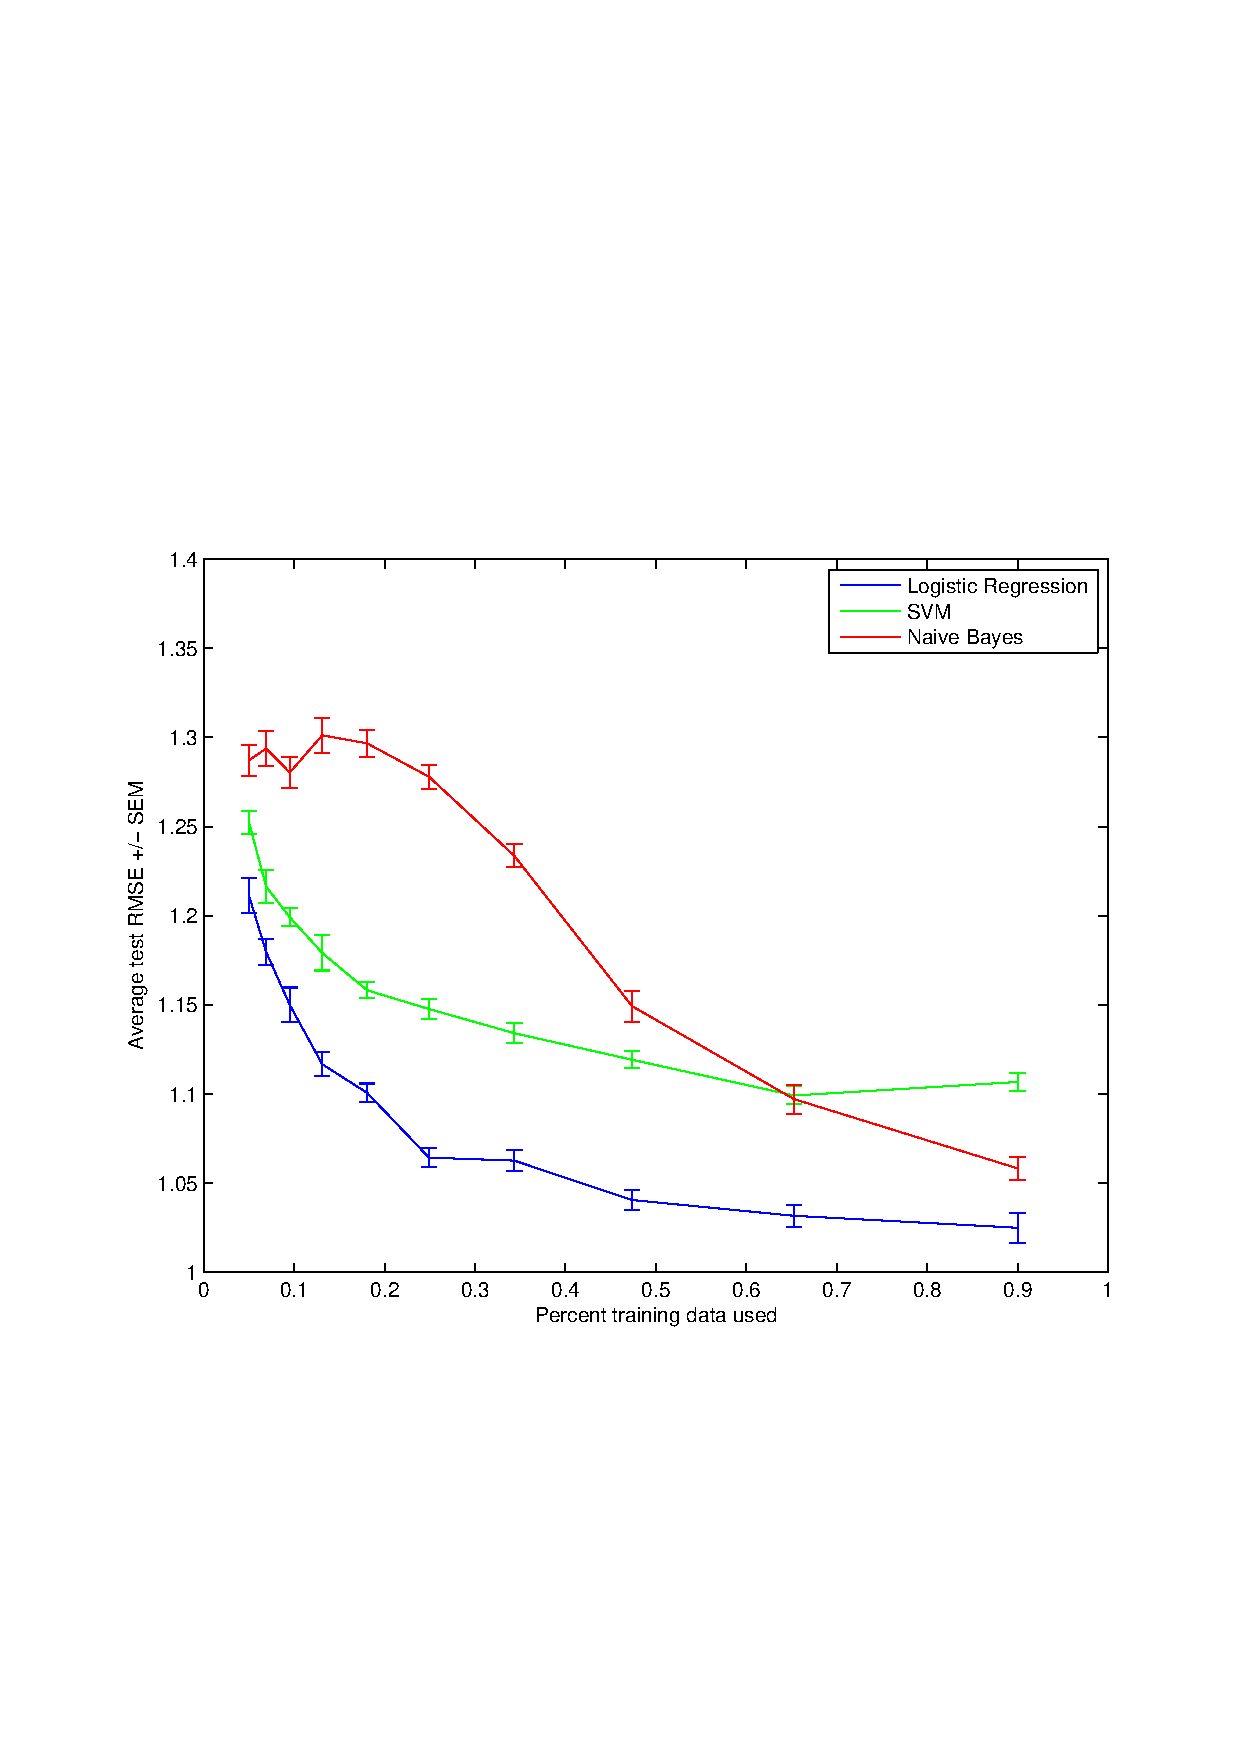
\includegraphics[width=\textwidth]{figs/rmse-nobs.pdf}
		\caption{RMSE performance of learners versus a 2500-sample holdout set versus size of training set. (Total training set size is 25,000, so test set size is a constant 0.1 percentage.)}
		\label{fig:rmsenobs}
	\end{subfigure}
	\quad
	\begin{subfigure}{.45\textwidth}
	\centering
		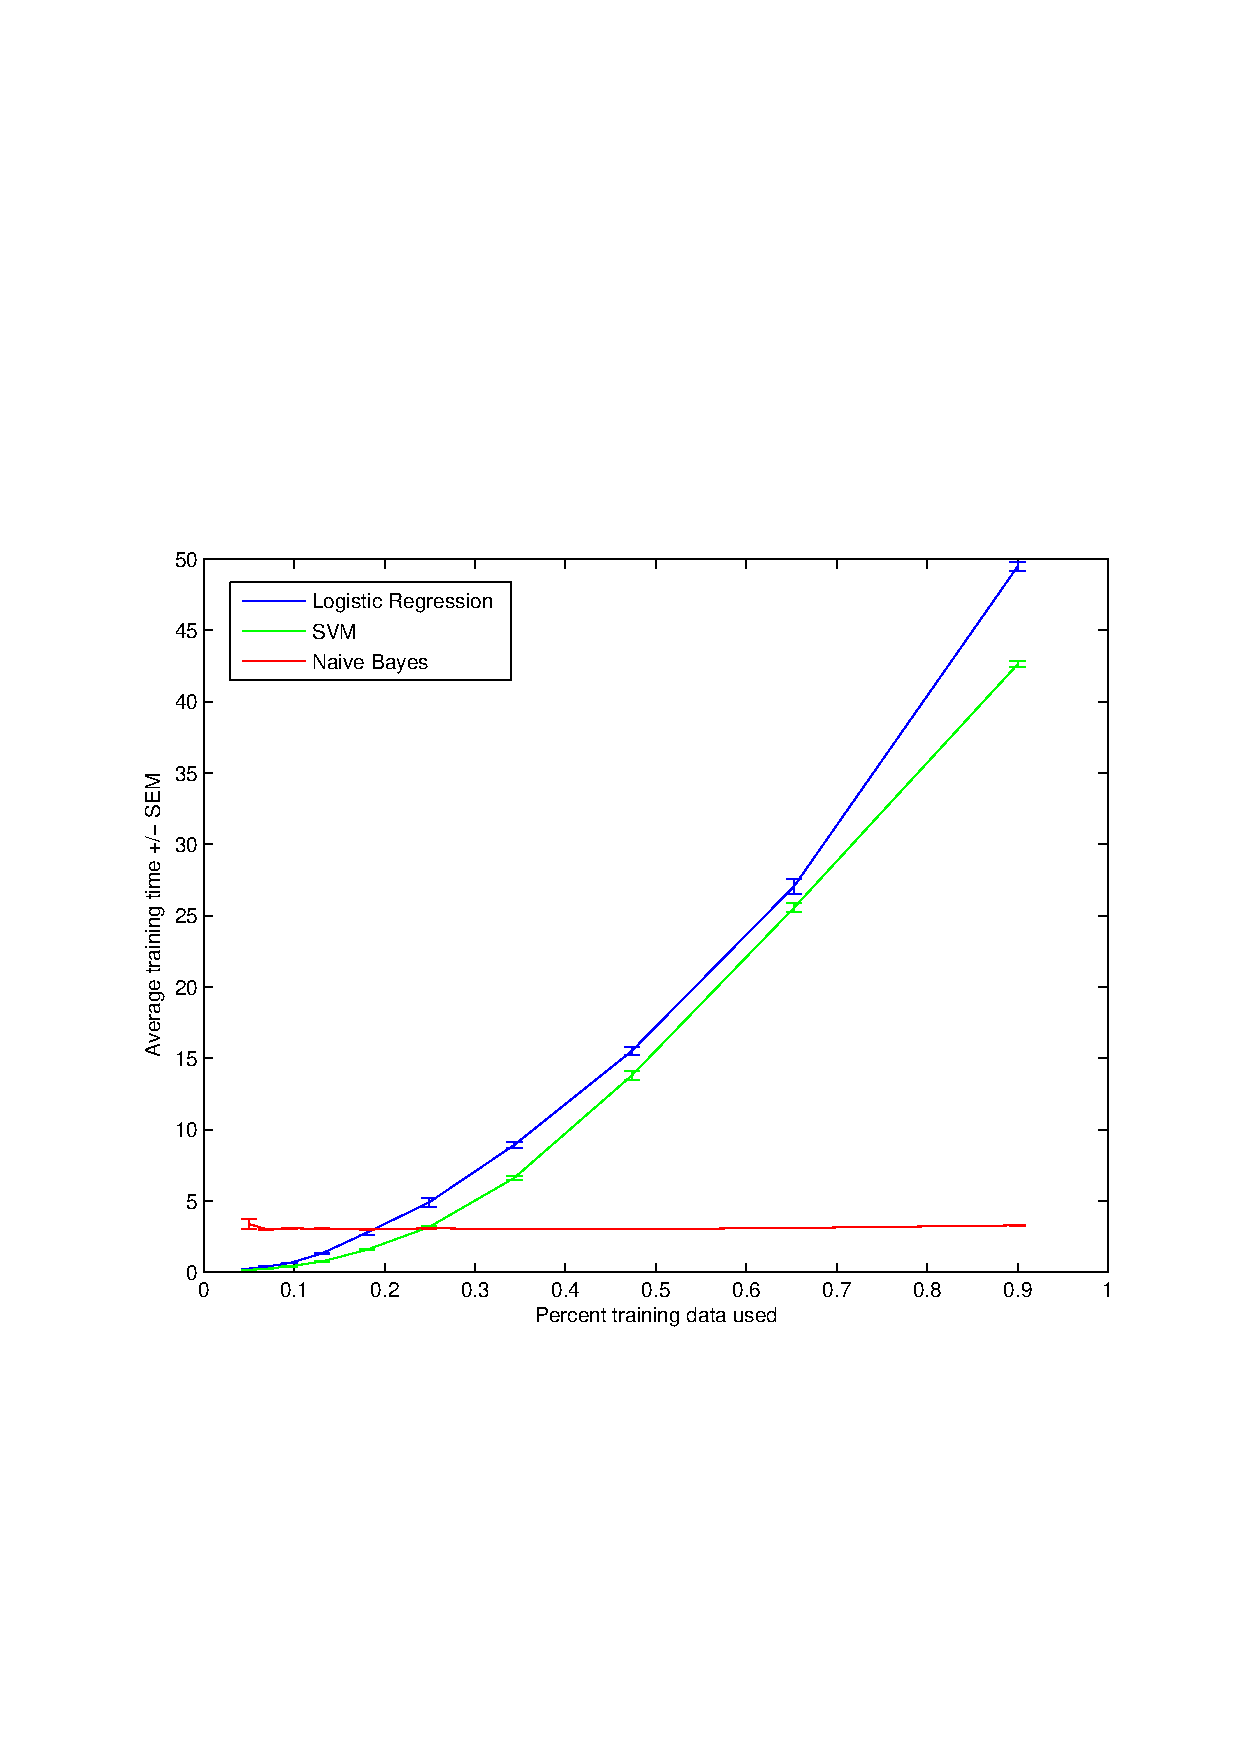
\includegraphics[width=\textwidth]{figs/time-nobs.pdf}
		\caption{Training time of learners (in sec) versus a 2500-sample holdout set versus size of training set. (Total training set size is 25,000, so test set size is a constant 0.1 percentage.)}
		\label{fig:timenobs}
	\end{subfigure}
	\caption{Behavior of learners with increased training set size}
\end{figure}

\subsection{�Unsuccessful� Learners}
\subsubsection{\texttt{eigenwords\_logit\_reg}}
Bigram matrices were generated from the combined training and quiz sets (using the complete text as found in the supplied metadata). We performed a singular value decomposition (SVD) on the bigram matrices, generating reduced-dimension left and right singular vectors (\textbf{U} and \textbf{V}, respectively) for each word in the vocabulary. Predictors for each document were the average position (centroid) of the document's words in the reduced-dimension space. This method was patterned off of Foster, Liberman, and Stine (unpublished)\footnote{``Featurizing Text: Converting Text into Predictors for Regression Analysis''. Dean P. Foster, Mark Liberman, and Robert A. Stine. Unpublished.}.

As revealed through cross-validation, prediction accuracy was, on average, was less than 30\%. As such, the performance of \texttt{eigenwords\_logit\_reg} was less than originally anticipated. We believe that the contrast between the performance found by Foster et al and us could be the result of a regression problem versus a classification problem, respectively, or a different performance metric: $R^2$ versus RMSE, respectively.

\subsubsection{\texttt{multi\_mira\_perceptron}}
A two-pass, multiclass perceptron/MIRA implementation derived from UC Berkeley CS 188\footnote{\url{http://inst.eecs.berkeley.edu/~cs188/fa09/projects/classification/classification.html}}
and CIS 520 lecture notes. The predictive accuracy for two passes was ~45\%; for three passes, almost 49\%. Ultimately, this learner was not used due to the amount of time necessary to train it, since for every review, the dot product of two large vectors needed to be computed per rating. Each vector was the size of the vocabulary lexicon, so each per review, $5 \times 56,835$ multiplications needed to take place, along with $5 \times 56,835$ resulting addition operations. For the training dataset in cross-validation ($N=10$), roughly $10 \times (2 \times 22,500 \times (5 \times 56,835)^2)$ operations needed to take place total.

\subsubsection{\texttt{kmeans}}
The top 75 principal components were selected using \matlab~built-in \texttt{svds}, and then fed into \texttt{kmeans} ($K=100$). The model then consisted of the centroids for the cluster, and the predicted rating for each cluster. The predicted rating of each cluster is determined by using the mean rating of all training data points that are members of that cluster. Predictions are done by taking the minimum euclidean distance between each test point and the clusters, and using the prediction for the minimally distanced cluster. Ultimately the distance metric used for the predictions needed major improving, primarily by using actual feature selection in order to do a like-for-like comparison of the test point to the cluster centroid. The mean RMSE during cross-validation of this classifier was on-par with \texttt{nb}/\texttt{counts\_svm}/counts\_logit, but the actual RMSE values swung a bit more wildly. Various $K$ values were tried, but none significantly improved the results.

\subsubsection{\texttt{business\_user\_classifier2}}
Unique index values were created for each business and user. These were then used to find the average rating value across all users for that business/user. To fill in missing values (businesses and users that were not in the training data), we used the average rating across all training data points. This method performed well in cross-validation, especially when paired with \texttt{counts\_logit\_reg}/\texttt{counts\_svm}/\texttt{nb}, it brought our mean RMSE down to $\sim 0.87$. However the approach sufferred from overfitting against the training data, as the performance against the quiz set dropped to $\sim 1.05$.

\subsubsection{\texttt{funny\_cool\_useful}}
This was a very simple 3-feature learner using the same logistic regression values as in \texttt{counts\_logit\_reg}. On its own, the cross-validation performance was around 1.5, but when paired with \texttt{counts\_logit\_reg}, \texttt{counts\_svm}, and \texttt{nb}, it offered a small but consistent boost to the cross-validation score. Ultimately we deferred testing it on quiz in favor of methods that may have offered larger improvements to the mean RMSE.

\section{Challenges}
\subsection{Dimensionality}
Due to the huge number of dimensions per review in the dataset, dimensionality reduction of some sort was needed in order to train certain classes of learners. For example, \matlab's built-in \texttt{kmeans} function was entirely unusable since we speculate within the function, it converts any sparse matrix passed into it into a full matrix. Any manipulations of the full matrix representation of the training dataset became all but impossible with a commodity piece of hardware like a MacBook. Moreover, we could not use \matlab�s built-in functions for principal component analysis like \texttt{pca} or \texttt{princomp}, as performing mean-centering on the sparse training data matrix converted it to a full matrix, which again, made it intractable to work with. One potential workaround we utilized to a varying degree of success involved simply performing SVD on a sparse matrix itself without mean centering, and taking the top $k + 1$ singular vectors. The first singular vector was discarded, and the rest were used as the top $k$ principal components. %***Maybe some analysis of why this did not perform too well? ***

\subsection{Final Learner}
The final learner used to generate predictions for the assessment test set consisted of \texttt{counts\_logit\_reg}, \texttt{nb}, \texttt{counts\_svm}. The resulting predicted rating from the three learners were combined using a weighted average with the following weights: $[0.417 0.368 0.172]$. The weights were determined experimentally through cross-validation ($N=10$), and observing that that weights produced via linear regression consistently produced the lowest, or second lowest RMSE for each round of cross-validation.

To meet the test set speed performance requirements with \matlab's built-in \texttt{NaiveBayes} functionality, a monkey-patched version was created which created that stored the output of \texttt{cell2mat(nb\_model.Params)} in \texttt{init\_models}. We then passed that stored value into the monkey-patched version of \texttt{predict.m}, which called into the monkey-patched version of \texttt{NaiveBayes.m}. This one change allowed us to boost our speed from $\sim8$ iterations/sec to $\sim 140$ iterations/sec.

Our performance against the quiz set with various learners in the final ensemble can be found in Table \ref{tab:quizperf}.

\begin{table}[h!]
\centering
\begin{tabular}{c c}
\hline
Learners & Mean RMSE \\ \hline\hline
\texttt{counts\_logit\_reg} & 1.0314 \\
\texttt{counts\_logit\_reg}, \texttt{nb} & 0.9723 \\
\texttt{counts\_logit\_reg}, \texttt{nb}, \texttt{counts\_svm} & 0.9548 \\
\texttt{counts\_logit\_reg}, \texttt{nb}, \texttt{counts\_svm}, \texttt{kmeans} & 0.9446 \\
\texttt{counts\_logit\_reg}, \texttt{nb}, \texttt{counts\_svm}, \texttt{business\_user\_classifier2} & 1.0413 \\\hline
\end{tabular}
\caption{Performance of various ensembles with the quiz set.}
\label{tab:quizperf}
\end{table}

%*** Brendan and/or Patrick ***
%If anyone has numbers for quiz performance, etc. saved we could insert a table here and talk more about performance metrics *** 

\section{Conclusion}
%*** What are people�s thoughts here? How could we improve our results, etc? ***
We performed reasonably well with 3 relatively simple classifiers: \nb, logistic regression, and support vector machines. Our performance was also consistent across cross-validation, against the quiz set, and against the test set, which shows we did not have any trouble with overfitting. Improved feature selection was one of the main areas that could have helped our results. It would have allowed us to run \texttt{kmeans} and get reasonable predictions at least. Additionally, creating some sort of similarity metric for comparing businesses/users would have been useful for filling in the businesses/users we had no prior knowledge of. Improving the n-gram creation to skip common stop words, or stemming the words before generating bigram matrices, may have improved the performance of the eigenword-based approaches.


\end{document}